% --------------------------------------------------------------
% This is all preamble stuff that you don't have to worry about.
% Head down to where it says "Start here"
% --------------------------------------------------------------

\title{Classifying the PFam dataset}
\author{Lionel Cheng}
\date{May 2022}

\documentclass[12pt]{article}

% Math
\usepackage{amsmath,amsthm,amssymb}
\usepackage{stmaryrd}

% Physics
\usepackage{physics}
\usepackage[version=4]{mhchem}
\usepackage{chemist}
\usepackage{siunitx}

% Other
\usepackage[margin=1in]{geometry}
\usepackage[utf8]{inputenc}
\usepackage[T1]{fontenc}
\usepackage{graphicx}
\usepackage{longtable}
\usepackage{booktabs}
\usepackage{array}
\usepackage{empheq}
\usepackage{enumitem}
\usepackage{scalerel}
\usepackage{subcaption}

% For bold upgreek letters
\usepackage{upgreek}
\usepackage{stmaryrd}
\SetSymbolFont{stmry}{bold}{U}{stmry}{m}{n}
\usepackage{bm}

% Bibliography
\usepackage{natbib}

\usepackage{xcolor}
\definecolor{linkcol}{rgb}{0,0,0.4}
\definecolor{citecol}{rgb}{0.5,0,0}
\definecolor{blue_sketch}{rgb}{0.1,0.1,0.4}
\definecolor{red_sketch}{rgb}{0.5,0,0}
\usepackage{hyperref}
\hypersetup{
    colorlinks=true,
    citecolor=citecol,
    linkcolor=linkcol,
    urlcolor=linkcol,
    linktoc=all
}

\newtheorem{definition}{Definition}[section]
\newtheorem{property}{Property}[section]
\newtheorem{theorem}{Theorem}[section]

% TikZ
\usepackage{tikz}
\usetikzlibrary{shapes.geometric, arrows}
\usetikzlibrary{calc}
\usepackage{algorithm2e}
% Commands related to ensembles
\newcommand{\N}{\mathbb{N}}
\newcommand{\Z}{\mathbb{Z}}
\newcommand{\R}{\mathbb{R}}
\newcommand{\C}{\mathbb{C}}
\newcommand{\Ltwo}[1]{\mathcal{L}^2(#1)}

% Intervals
\newcommand{\intint}[2]{\llbracket #1, #2 \rrbracket}

% Vectors/Tensors and bold symbols
\newcommand{\ve}[1]{\vb*{#1}}
\newcommand{\x}{\vb{x}}
\newcommand{\vr}{\vb{r}}
\newcommand{\vv}{\vb{v}}
\newcommand{\kv}{\vb{k}}
\newcommand{\av}{\vb{a}}
\newcommand{\U}{\vb{U}}
\newcommand{\uv}{\vb{u}}
\newcommand{\er}{\vb{e}_r}
\newcommand{\et}{\vb{e}_\theta}
\newcommand{\vt}{\vb{t}}
\newcommand{\vF}{\vb{F}}
\newcommand{\ex}{\vb{e}_x}

% Derivatives
\newcommand{\dtadv}[2]{\frac{\delta #1}{\delta #2}}
\newcommand{\ut}{\pdv{u}{t}}
\newcommand{\ux}{\pdv{u}{x}}
\newcommand{\uxx}{\pdv[2]{u}{x}}

% Operators
\newcommand{\hf}{\hat{f}}
\newcommand{\hu}{\hat{u}}
\newcommand{\e}{\mathrm{e}}
\newcommand{\ii}{\mathrm{i}}
\newcommand{\F}{\mathcal{F}}
\newcommand{\I}{\mathrm{I}}

% Capital greek letters not in italic (delta and omega)
\DeclareMathSymbol{\upD}{\mathalpha}{operators}{1}
\DeclareMathSymbol{\upP}{\mathalpha}{operators}{5}
\DeclareMathSymbol{\upS}{\mathalpha}{operators}{6}
\DeclareMathSymbol{\upO}{\mathalpha}{operators}{10}
\newcommand{\dt}{\upD t}
\newcommand{\dx}{\upD x}
\newcommand{\dy}{\upD y}
\newcommand{\lapl}{\upD}

% Finite element
\newcommand{\sumfe}{\sum_{\tau \in E(i)} \sum_{k \in \tau}}
\newcommand{\sumcell}{\sum_{\tau \in E(i)}}

% Redefinition (more compact)
\newcommand{\veps}{\varepsilon}
\newcommand{\eps}{\epsilon}
\newcommand{\psc}{\scaleto{\partial}{5pt}}
\newcommand{\mrm}{\mathrm}
\newcommand{\mc}{\mathcal}
\newcommand{\ta}{\theta}
\newcommand{\tij}{t_{ij}}
\newcommand{\phij}{\phi_{i, j}}
\newcommand{\tS}{\tilde{S}}
\newcommand{\tN}{\tilde{N}}
\newcommand{\tR}{\tilde{R}}
\newcommand{\tin}{\mathrm{in}}
\newcommand{\out}{\mathrm{out}}

% Misc (rather long formulas)
\newcommand{\green}{G(\vb{x}, \vb{x}')}
\newcommand{\cylgrad}[3]{\dfrac{\partial #1}{\partial r} + \dfrac{1}{r} \dfrac{\partial #2}{\partial \theta} + \dfrac{\partial #3}{\partial z}}
\newcommand{\cyldiv}[3]{\dfrac{1}{r}\dfrac{\partial r #1}{\partial r} + \dfrac{1}{r} \dfrac{\partial #2}{\partial \theta} + \dfrac{\partial #3}{\partial z}}

% Quantum mechanics
\newcommand{\mean}[1]{\langle #1 \rangle}
\newcommand{\wf}{\psi(\ve{r}, t)}
\newcommand{\ham}{\hat{H}}
\newcommand{\hA}{\hat{A}}
\newcommand{\hB}{\hat{B}}
\newcommand{\upd}{\mathrm{d}}
\newcommand{\psia}{\psi_\alpha(\ve{r})}
\newcommand{\kpsi}{\ket{\psi}}
\newcommand{\bpsi}{\bra{\psi}}
\newcommand{\kb}{\ket{n}}
\newcommand{\knr}{\ket{n, r}}
\newcommand{\kpsiz}{\ket{\psi^0}}
\newcommand{\kpsio}{\ket{\psi^1}}
\newcommand{\kpsit}{\ket{\psi^2}}
\newcommand{\hv}[1]{\hat{\vb*{#1}}}
\newcommand{\hvr}{\hat{\vb{r}}}
\newcommand{\vp}{\vb*{p}}
\newcommand{\hvp}{\hat{\vb*{p}}}
\newcommand{\kpsin}{\ket{\psi_n}}
\newcommand{\bpsin}{\bra{\psi_n}}
\newcommand{\hO}{\hat{O}}

% Statistical Physics and kinetic theory
\newcommand{\Ni}{\mathcal{N}_i}
\newcommand{\NN}{\mathcal{N}}
\newcommand{\Qrot}{\mathcal{Q}^\text{rot}}
\newcommand{\Q}{\mathcal{Q}}
\newcommand{\evibsnv}{\epsilon_\text{s,nv}^\text{vib}}
\newcommand{\erotsnv}{\epsilon_\text{s,nv}^\text{rot}}
\newcommand{\evib}{\varepsilon_\text{vib}}
\newcommand{\eR}{\varepsilon_R}
\newcommand{\fastp}{\dot{E}^p_\text{fast}}
\newcommand{\vibp}{\dot{E}^p_\text{vib}}
\newcommand{\vfone}{\vb{f}_{1}}
\newcommand{\di}{\mathrm{d}}
\newcommand{\tA}{\mathrm{A}}
\newcommand{\tBC}{\mathrm{BC}}
\newcommand{\vib}{\text{vib}}
\newcommand{\Ntwo}{\ce{N2}}
\newcommand{\Otwo}{\ce{O2}}
\newcommand{\qlpl}{\{q_l, p_l\}}
\newcommand{\dqdp}{\prod_l dq_l dp_l}

% Relaxation times
\newcommand{\tautt}{\tau_\text{TT}}
\newcommand{\taurt}{\tau_\text{RT}}
\newcommand{\tauvt}{\tau_\text{VT}}
\newcommand{\Erot}{E_\text{rot}}
\newcommand{\Evib}{E_\text{vib}}

% Metric related properties
\newcommand{\dvi}{\partial V_i}
\newcommand{\Sij}{\vb{S}_{i, j}^\tau}
\newcommand{\Si}{\vb{S}_i^\tau}
\newcommand{\pipe}[1]{\left. #1 \right\vert}

% Units
\newcommand{\ns}{\SI{}{\nano\second}}
\newcommand{\mus}{\SI{}{\micro\second}}
\newcommand{\ms}{\SI{}{\milli\second}}
\newcommand{\kHz}{\SI{}{\kilo\hertz}}

% Small partial in integrals
\newcommand\ppartial{\scaleobj{0.7}{\partial}}

% Differential
\newcommand{\md}{\mrm{d}}

% Environnement pour insérer une image en dehors des marges - bigcenter
\makeatletter
\newskip\@bigflushglue \@bigflushglue = -200pt plus 1fil
\def\bigcenter{\trivlist \bigcentering\item\relax}
\def\bigcentering{\let\\\@centercr\rightskip\@bigflushglue%
	\leftskip\@bigflushglue
	\parindent\z@\parfillskip\z@skip}
\def\endbigcenter{\endtrivlist}

\newcommand\highlight[1]{{\textcolor{red}{#1}}}

% Theorems and definitions

\begin{document}
\maketitle

% --------------------------------------------------------------
%                         Start here
% --------------------------------------------------------------

\section{Dataset Analysis}

\subsection{Overview of the dataset}

The PFam dataset \cite{Mistry2020} is a widely used resource for classifying protein sequences into families and domains. It is used by experimental biologists researching specific proteins, by structural biologists to identify new targets for structure determination, by computational biologists to organise sequences and by evolutionary biologists tracing the origins of proteins.

Deep learning has been applied on such datasets in \cite{Bileschi2022}. The purpose of the dataset in this report is to repose the PFam seed dataset as a multiclass classification machine learning task.

The task is: given the amino acid sequence of the protein domain, predict which class it belongs to. There are about 1 million training examples, and 18,000 output classes.

The dataset has been randomly splitted into a training, validation and test datasets. The first entries of the training datasets are shown in Tab.~\ref{tab:training_head_5}. For each entry corresponding to a protein domain, 5 properties are found: family\_id, sequence\_name, family\_accesion, aligned\_sequence and sequence.

\begin{itemize}
    \item sequence\_name is a unique identifier for the sequence
    \item family\_id and family\_accesion correspond to the labels of our dataset
    \item sequence correspond to the list of amino-acids of the sequence
    \item aligned\_sequence contains a single sequence from the multiple sequence alignment generated using hidden Markov models \citep{Finn_2007}
\end{itemize}

\begin{table}[htbp]
    \footnotesize
    \begin{tabular}{lllll}
    \toprule
          family\_id &        sequence\_name & family\_accession &                                   aligned\_sequence &                                           sequence \\
    \midrule
    Penicillinase\_R &   Q81U16\_BACAN/8-123 &       PF03965.16 & ISEAELEIMK & ISEAELEIMK \\
             Rtt106 &   POB3\_CANAL/362-454 &       PF08512.12 & AGVPCSVKA. & AGVPCSVKAS \\
      F-actin\_cap\_A &  Q8I3I2\_PLAF7/12-301 &       PF01267.17 & IRHVLMNSPP & IRHVLMNSPP \\
          HupF\_HypC &    O28902\_ARCFU/1-65 &       PF01455.18 & MCIAIPGR.. & MCIAIPGRIE \\
            DUF3794 & R6BY75\_9CLOT/189-271 &        PF12673.7 & NIFHI..LWE & NIFHILWEDV \\
    \bottomrule
\end{tabular}
\caption{Example of the first 5 entries of the training dataset. The aligned\_sequence and sequence entries have been cropped to the first 10 amino-acids.}
\label{tab:training_head_5}
\end{table}

The dataset has been splitted so that 80\% is contained in the training dataset and 10\% in the validation and test datasets respectively. The number of sequences, the number of unique families and the number of unique amino-acids can be found in Tab.~\ref{tab:dsets_description} for each dataset. We see that the number of families and amino-acids is not the same depending on the dataset: this should be taken into account during training.

\begin{table}[htbp]
    \centering
    \begin{tabular}{llll}
        \toprule
        Partition & Number of sequences & Number of unique families & Number of amino acids \\
        \midrule
        Train & 1086741 & 17929 & 25 \\
        Valid & 126171 & 13071 & 22 \\
        Test & 126171 & 13071 & 24 \\
        \bottomrule
    \end{tabular}
    \caption{Description of the global properties of the three datasets.}
    \label{tab:dsets_description}
\end{table}

\subsection{Dataset metrics}

The distribution of the 20 most common labels in the datasets is shown in Fig.~\ref{fig:labels_dist} for the three datasets. We can confirm that the random split has been well performed since the proportion of each dataset is conserved across the shown families (this has also been checked across the other families).

\begin{figure}[htbp]
    \centering
    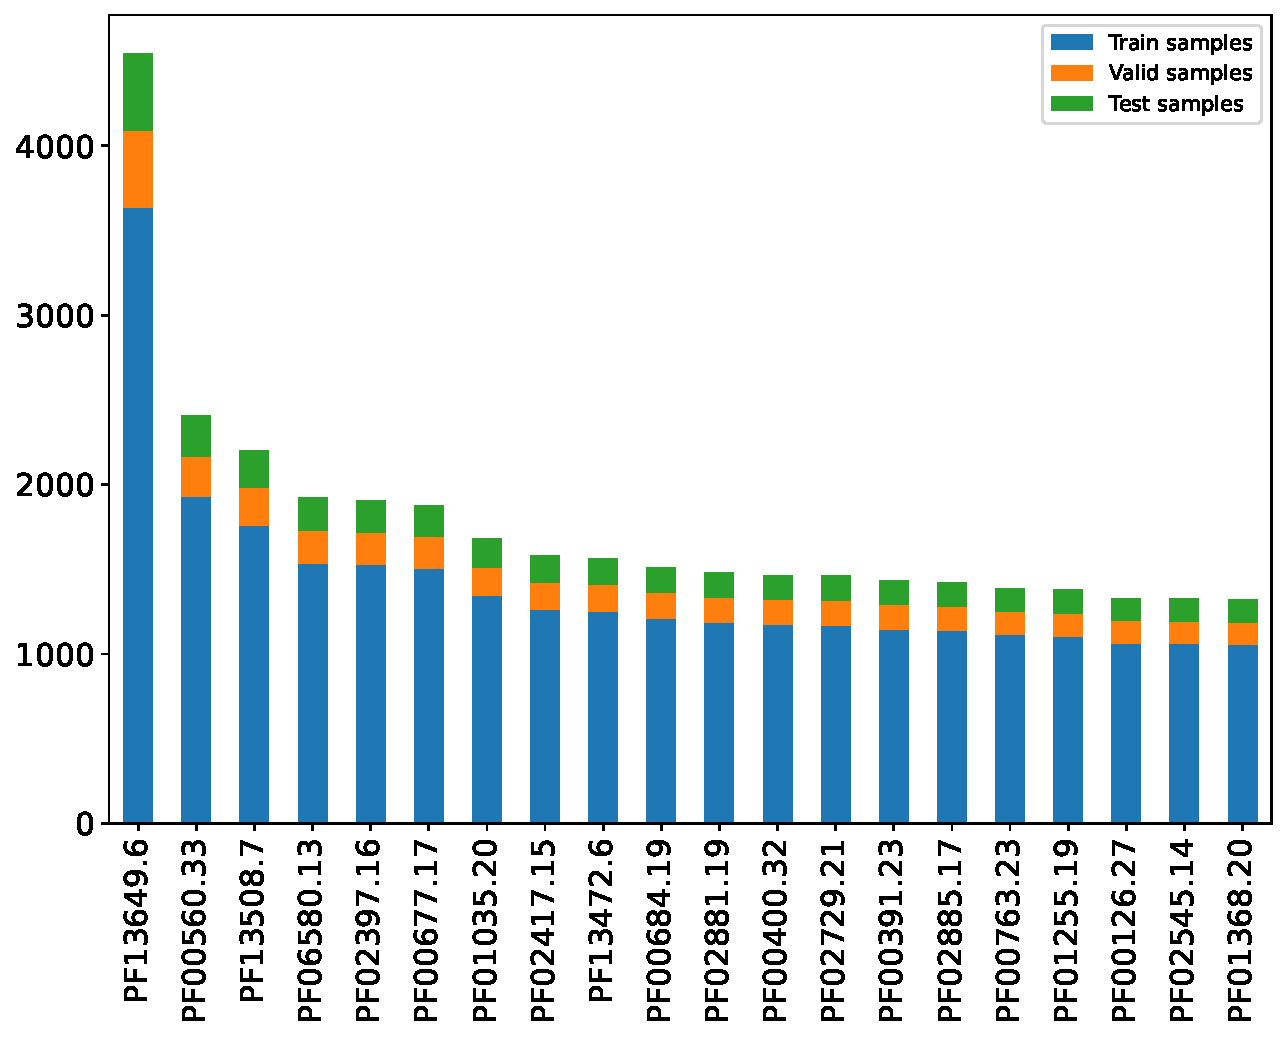
\includegraphics[width=0.6\textwidth]{figures/labels_dist.pdf}
    \caption{Distribution of the 20 most common labels.}
    \label{fig:labels_dist}
\end{figure}

We now turn to the length of the sequences which is not uniform across the datasets as shown in Fig.~\ref{fig:length_dist}. The distributions are again close to each other and we can see that most of the sequences have a length around 100.

\begin{figure}[htbp]
    \centering
    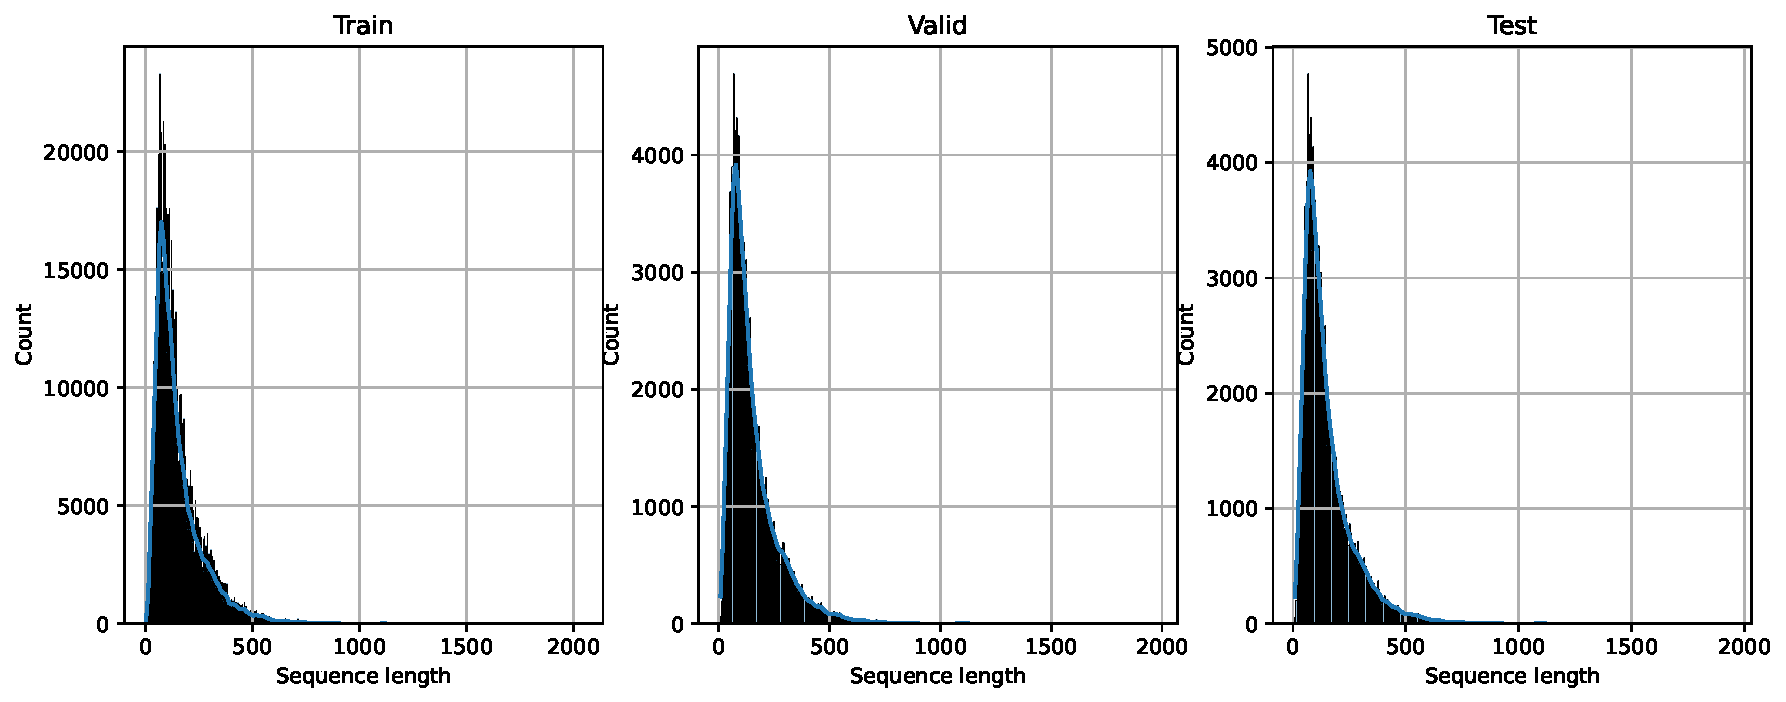
\includegraphics[width=\textwidth]{figures/length_seq.pdf}
    \caption{Distribution of the length of the sequences in each dataset.}
    \label{fig:length_dist}
\end{figure}

Finally the distribution of the amino-acids in each dataset is shown in Fig.~\ref{fig:aminoacids_dist}. As said earlier, there are 25, 22 and 24 amino acids in the train, validation and test datasets respectively and the 20 most common ones are the same across the three datasets: these are the 20 most common amino-acids in nature \citep{twenty_aminoacids}. The other amino acides present in the sequences (X, U, B, O, Z) are really rare and seem to not be really relevant for classification.

\begin{figure}[htbp]
    \centering
    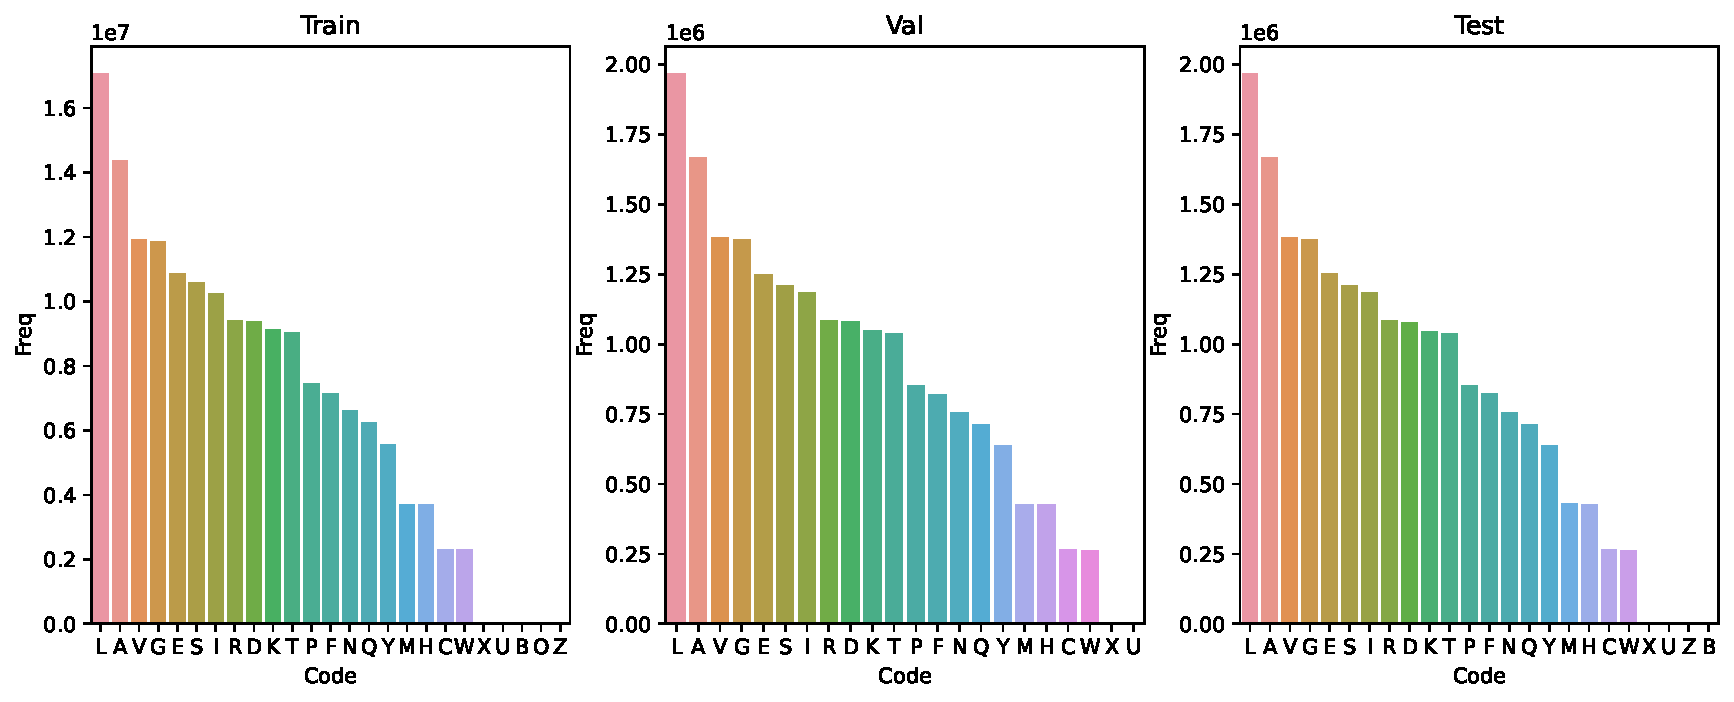
\includegraphics[width=\textwidth]{figures/amino_acids_dist.pdf}
    \caption{Distribution of the amino acids in each dataset.}
    \label{fig:aminoacids_dist}
\end{figure}

\subsection{Dataset families}

This section focuses on families of the dataset and tries to understand what is unique in each family. These properties should be, one way or another, be understood by the neural network. We choose two families from the 20 most common families in the datasets in Fig.~\ref{fig:labels_dist}: the PF13649.6 and PF00677.17 families. For each one the sequence length distribution and the transition matrix heatmap are plotted in Figs.~\ref{fig:13649_props} and \ref{fig:00677_props}. The transition matrix should be read as follows: for each row (associated to a letter) each column correspond to the probability that the next letter is one of the column. Hence for the PF13649.6 family the C amino-acid is mostly followed by the G amino-acid in Fig.~\ref{fig:13649_props_hm}.

For each family we can see there is a certain coherence in terms of sequence length for each family: all sequences of a family have similar sequence lengths for the most-common labels. The transition matrix can be considered as a unique footprint of each family.

\begin{figure}[htbp]
    \centering
    \begin{subfigure}{\textwidth}
        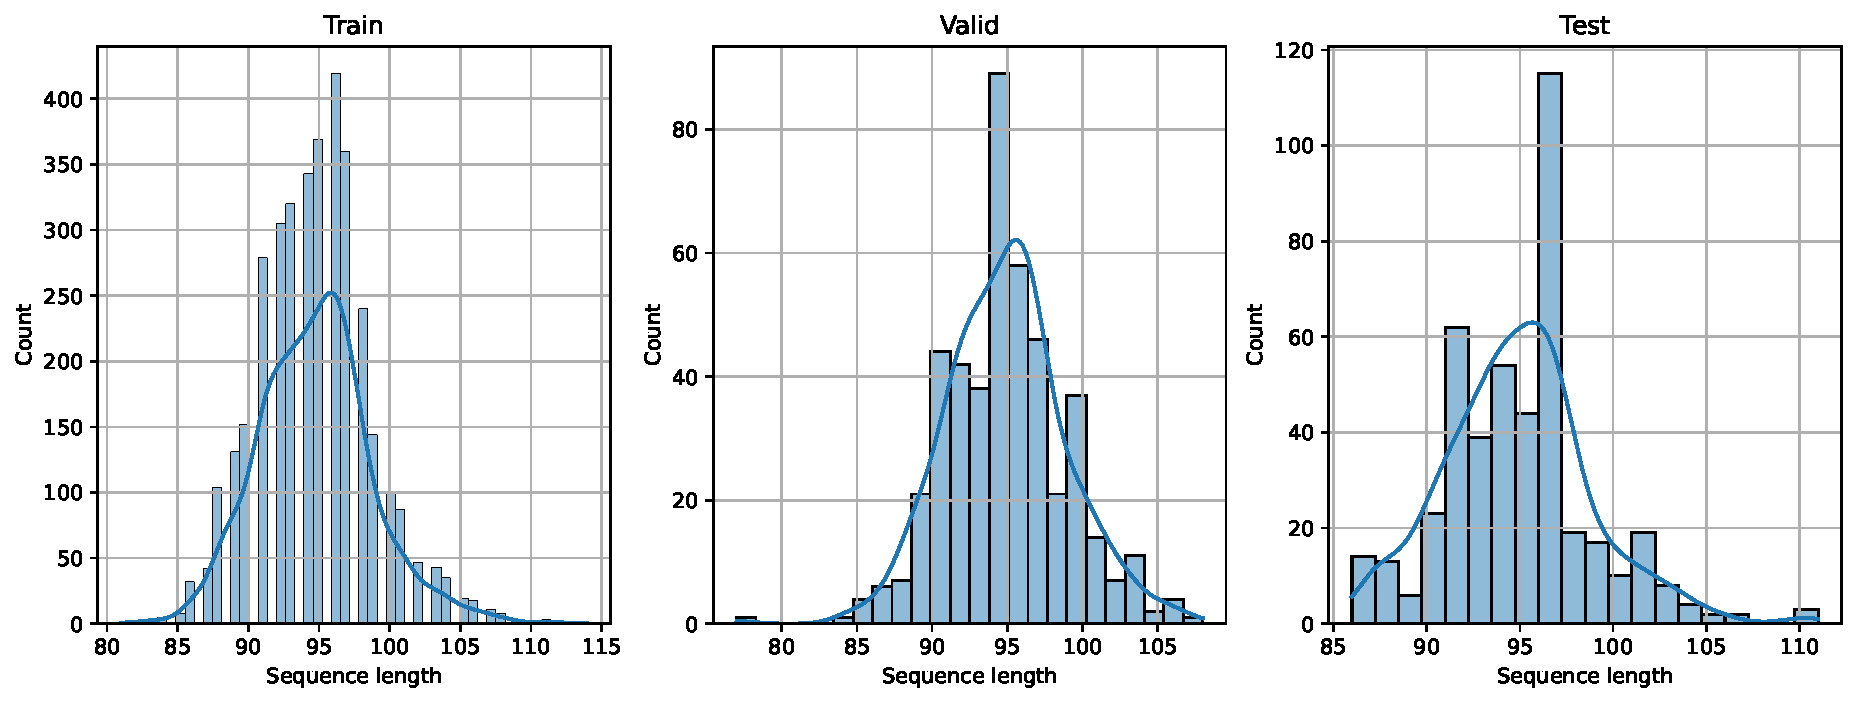
\includegraphics[width=\textwidth]{figures/length_seq_13649.pdf}
        \caption{Length distribution}
    \end{subfigure}
    \begin{subfigure}{0.5\textwidth}
        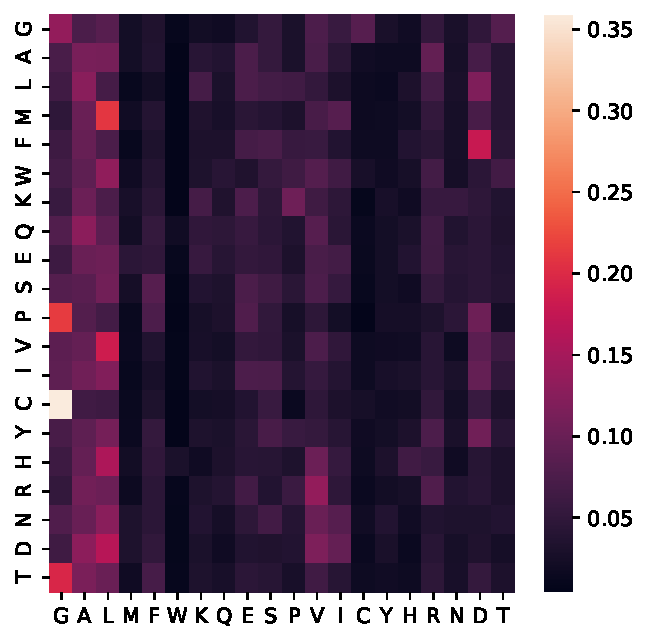
\includegraphics[width=\textwidth]{figures/seq_heatmap_13649.pdf}
        \caption{Transition Matrix Heatmap in train dataset}
        \label{fig:13649_props_hm}
    \end{subfigure}
    \caption{Properties of the PF13649.6 family.}
    \label{fig:13649_props}
\end{figure}

\begin{figure}[htbp]
    \centering
    \begin{subfigure}{\textwidth}
        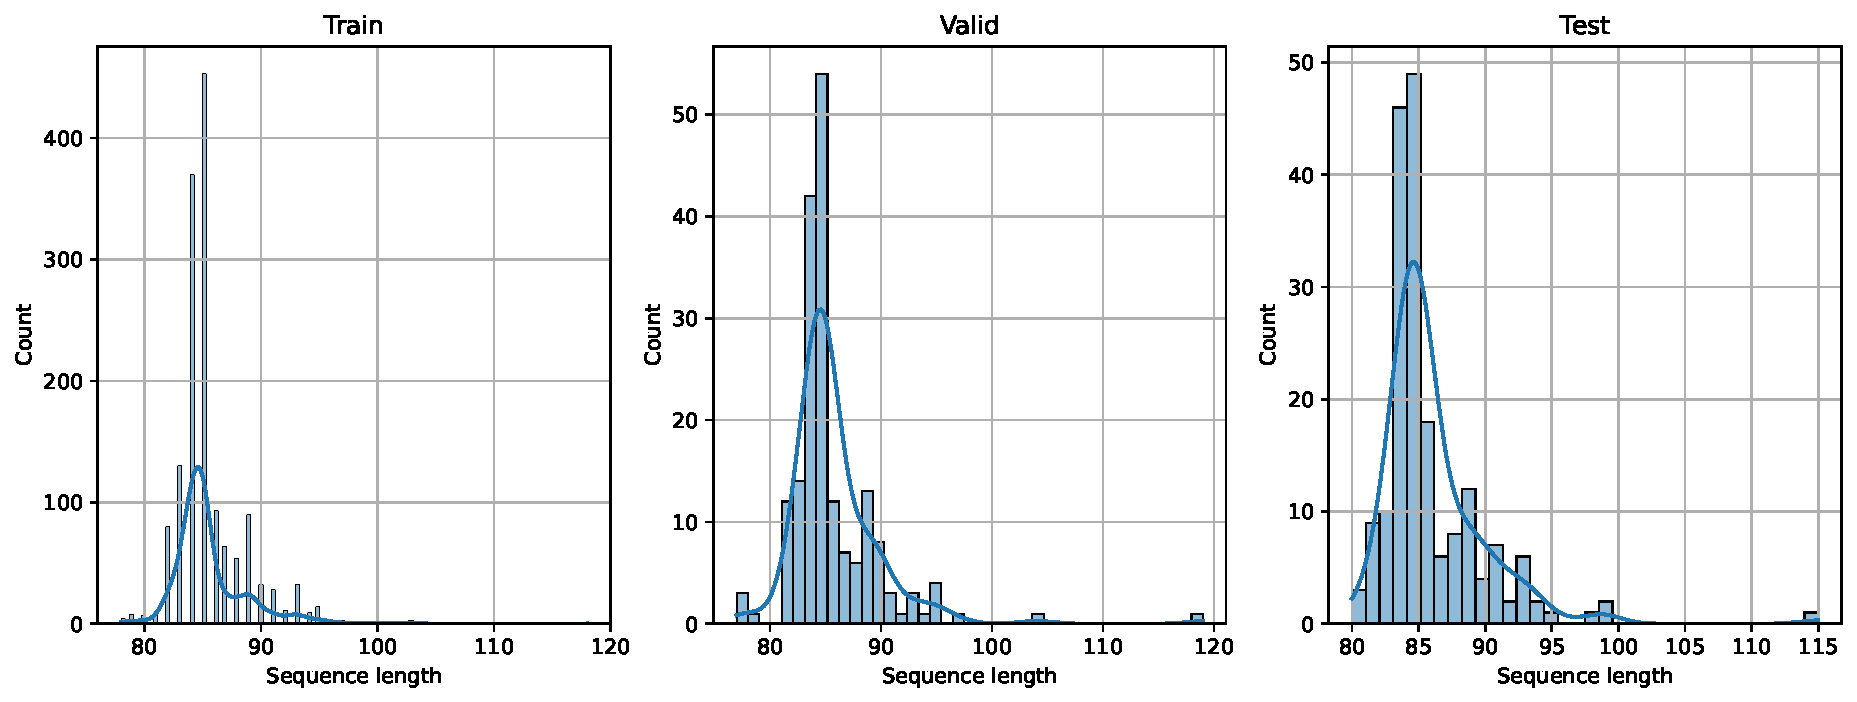
\includegraphics[width=\textwidth]{figures/length_seq_00677.pdf}
        \caption{Length distribution}
    \end{subfigure}
    \begin{subfigure}{0.5\textwidth}
        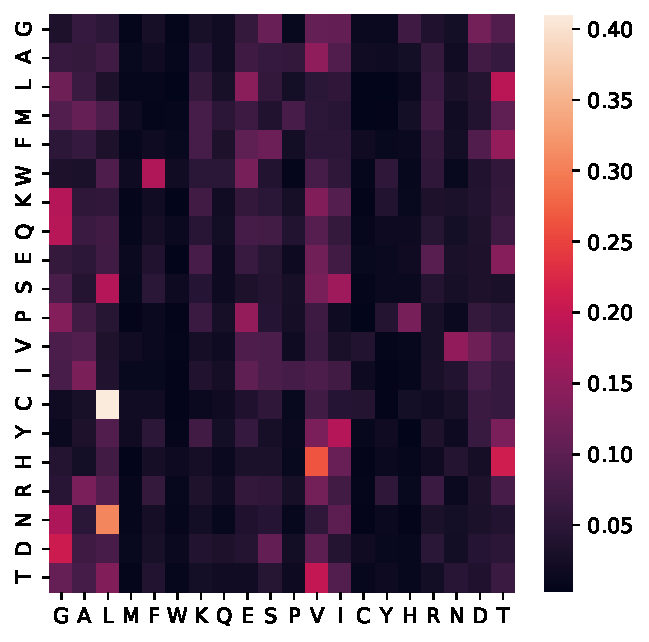
\includegraphics[width=\textwidth]{figures/seq_heatmap_00677.pdf}
        \caption{Transition Matrix Heatmap in train dataset}
    \end{subfigure}
    \caption{Properties of the PF00677.17 family.}
    \label{fig:00677_props}
\end{figure}

\section{Method Explanation}

The method used to tackle this classification problem is now explained. The whole code is written using the PyTorch library. First the dataset is reduced and encoded to homogeneize entries and make it suitable for training. Then the neural network architecture is discussed as well as the loss and optimizer used.

\subsection{Dataset reduction and encoding}

From the dataset analysis performed above, we use 3 parameters to reduce the dataset: the number of common labels $n_\mrm{mc}$, the maximum length of the sequences $l_\mrm{max}$ and the number of amino acids classes $n_\mrm{aa}$.

The number of common labels $n_\mrm{mc}$ allows to decrease the complexity of the classification problem so that it is easy to test that everything is working properly before scaling up. We choose the number of most common labels in the \textbf{training} dataset and filter the three datasets to include only the sequences whose labels are among this set. The labels are each assigned an integer to create a unique identifier for each label.

As shown in Fig.~\ref{fig:aminoacids_dist}, only 20 amino-acids are really meaningful in this dataset. We create a letter to integer (1 to 20) correspondance to encode each of these 20 amino-acid and set all the other amino acids to 0.

The length of the sequences in the datasets is not constant (Fig.\ref{fig:length_dist}) and it would be easier to have constant length sequences. To do so we set the maximum length of the sequences to $l_\mrm{max}$ by cutting the sequences or adding padding zeros to the encoded sequences.

Finally the  labels are each assigned an integer

All these treatments are done in the \texttt{ProteinDataset} class in the \texttt{dataset.py} file of the \texttt{proteinclass} library.

\subsection{Neural network architecture}

After dataset reduction and encoding the input matrix $\vb{X}$ of a neural network and the target labels $\vb{y}$ have the following shape:

\begin{equation}
    \vb{X} = \begin{bmatrix}
        x_{1,1} & \ldots & \ldots & x_{1,l_\mrm{max}} \\
        \vdots & \ldots & \ldots & \vdots \\
        x_{b_s,1} & \ldots & \ldots & x_{b_s,l_\mrm{max}} \\
    \end{bmatrix} \in \intint{0}{20}^{b_s \times l_\mrm{max}},
    \quad
    \vb{y} = \begin{bmatrix}
        y_1 \\ \vdots \\ y_{b_s}
    \end{bmatrix}
    \in \intint{0}{n_\mrm{mc} - 1}^{b_s}
\end{equation}

\noindent where $b_s$ is the batch-size. Each row in this matrix corresponds to an encoded sequence that has been padded to $l_\mrm{max}$ length. At this point the input matrix could be encodded in two ways in the first layer of the neural network: by using a one-hot encoding or a word embedding. The size of the vocabulary (in our case the number of amino-acids) being relatively small (21), there is no curse of dimensionality using the one-hot encoding. We expect certain amino-acids to be more closely related than others and a one-hot encoding can not capture that as it imposes orthogonality between all the amino-acids.

We thus begin our networks with an embedding layer (\texttt{nn.Embedding} in the code) where the embedding dimension is $n_e$. The simplest network (\texttt{SimpleProteinClass} class in \texttt{model.py} file of the \texttt{proteinclass} library) is followed by a fully-connected (FC) layer so that the network is depicted in Fig.~\ref{fig:simple_network}.

\begin{figure}[htbp]
    \centering
    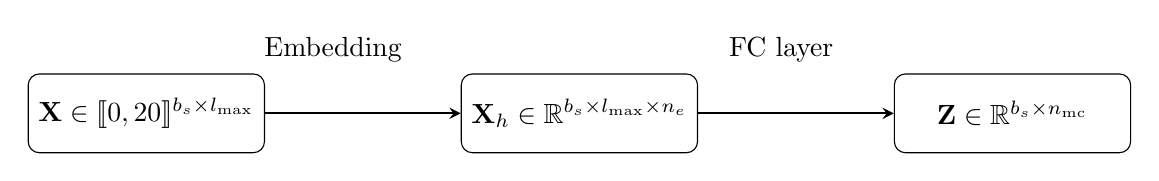
\begin{tikzpicture}[node distance=1.5cm]
    \tikzstyle{arrow} = [thick, ->, >=stealth]
    \tikzstyle{neuralnetwork} = [rectangle, rounded corners, minimum width=3cm, minimum height=1cm, text centered, draw=black, fill=white]

    \tikzstyle{plasmatransport} = [rectangle, rounded corners, minimum width=3cm, minimum height=1cm, text centered, draw=black, fill=white]
    % Blocks
    \node (nn) [neuralnetwork, xshift=-1.0cm] {$\vb{X} \in \intint{0}{20}^{b_s \times l_\mrm{max}}$};
    \node (plasmat) [plasmatransport, xshift=4.0cm, right of=nn] {$\vb{X}_h \in \R^{b_s \times l_\mrm{max} \times n_e}$};
    \node (final) [neuralnetwork, xshift=4.0cm, right of=plasmat] {$\vb{Z} \in \R^{b_s \times n_\mrm{mc}}$};

    % Arrows
    \draw [arrow] (nn) -- node[text width=2.5cm,midway,above=1.5em]{Embedding} (plasmat);
    \draw [arrow] (plasmat) -- node[text width=2.5cm,midway,above=1.5em, xshift=0.4cm]{FC layer} (final);

\end{tikzpicture}
    \caption{\texttt{SimpleProteinClass} network.}
    \label{fig:simple_network}
\end{figure}

This very simple network has the caveat of having a lot of parameters since the fully convolutional layers directly flattens the embedding matrix. To reduce the memory footprint of the model, we design two other models which add another layer after the embedding and before the FC layer: the \texttt{RNNProteinClass} which add one or more Recurent Neural Network (RNN) layers and \texttt{LSTMProteinClass} which add one or more Long Short Term Memory (LSTM) layers. This decreases greatly the number of parameters although it is more computationaly expensive.

\begin{figure}[htbp]
    \centering
    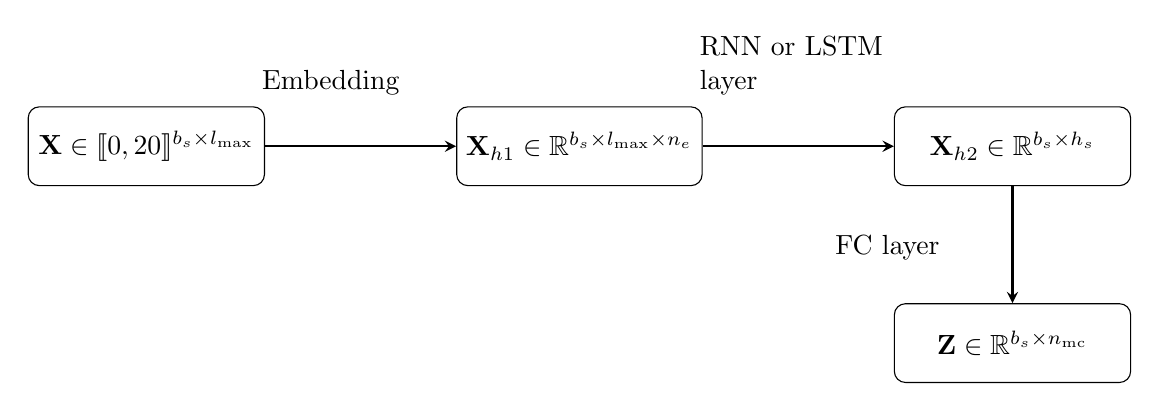
\begin{tikzpicture}[node distance=1.5cm]
    \tikzstyle{arrow} = [thick, ->, >=stealth]
    \tikzstyle{neuralnetwork} = [rectangle, rounded corners, minimum width=3cm, minimum height=1cm, text centered, draw=black, fill=white]

    \tikzstyle{plasmatransport} = [rectangle, rounded corners, minimum width=3cm, minimum height=1cm, text centered, draw=black, fill=white]
    % Blocks
    \node (nn) [neuralnetwork, xshift=-1.0cm] {$\vb{X} \in \intint{0}{20}^{b_s \times l_\mrm{max}}$};
    \node (plasmat) [plasmatransport, xshift=4.0cm, right of=nn] {$\vb{X}_{h1} \in \R^{b_s \times l_\mrm{max} \times n_e}$};
    \node (hidden) [plasmatransport, xshift=4.0cm, right of=plasmat] {$\vb{X}_{h2} \in \R^{b_s \times h_s}$};
    \node (final) [neuralnetwork, yshift=-1.0cm, below of=hidden] {$\vb{Z} \in \R^{b_s \times n_\mrm{mc}}$};

    % Arrows
    \draw [arrow] (nn) -- node[text width=2.5cm,midway,above=1.5em]{Embedding} (plasmat);
    \draw [arrow] (plasmat) -- node[text width=2.5cm,midway,above=1.5em, xshift=0.cm]{RNN or LSTM layer} (hidden);
    \draw [arrow] (hidden) -- node[text width=2.5cm,midway,above=0.5em, xshift=-1.0cm, yshift=-0.5cm]{FC layer} (final);
\end{tikzpicture}
    \caption{\texttt{RNNProteinClass} and \texttt{LSTMProteinClass} networks.}
    \label{fig:medium_network}
\end{figure}

\subsection{Loss and optimizer}

We use a simple stochastic gradient optimizer \citep{ruder2016} for the optimizer and the loss is the classical cross-entropy loss for categorical data \citep[Chap. 4]{bishop}:

\begin{equation}
    l(\vb{Z}, \vb{y}) = \frac{1}{b_s} \sum_{b=1}^{b_s} - \log \frac{\exp(Z_{b, y_b})}{\sum_{n=1}^{n_\mrm{mc}} \exp(Z_{b, n})}
\end{equation}

\noindent where $\vb{Z}$ is the output after the FC layer in Fig.~\ref{fig:simple_network}.

\section{Experiment Description}

To be able to easily debug and understand the network behavior on the dataset we vary the $n_\mrm{mc}$ parameter, \textit{i.e.} the number of most-common labels in the training dataset used to filter the datasets. The small set will consist of only the 200 most common labels and will be used to test the different networks architectures and tune the hyperparameters. The medium set contains 5000 labels.

\section{Result Analysis}

\subsection{Small set}

We start by tuning the optimizer parameters of the different network architectures on the 200 labels dataset. The training set contains now 156 275 entries, the validation and test 19 426 entries. We vary two parameters that control the optimization: the learning rate and the maximum norm of gradient (above which it is clipped).

The \texttt{SimpleProteinClass} is first tested by setting the maximum norm of gradient to 5 and varying the fixed learning rate from 0.001 to 1.0. The embedding size of the first layer is set to 40 so that the network contains 801 040 trainable parameters. The training and validation loss/accuracy are shown in Fig.~\ref{fig:loss_acc_simple200labels}: the optimal value of the learning rate for this case is between 0.1 and 1.0.

\begin{figure}[htbp]
    \centering
    \begin{subfigure}{\textwidth}
        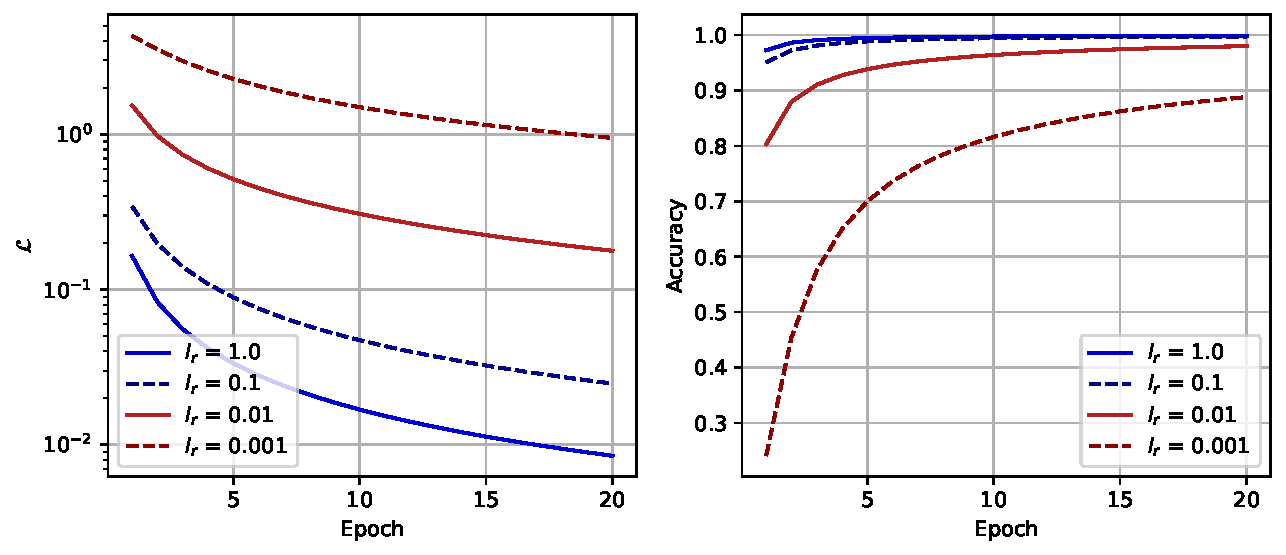
\includegraphics[width=\textwidth]{figures/loss_acc_simple200labels_train.pdf}
        \caption{Training dataset}
    \end{subfigure}
    \begin{subfigure}{\textwidth}
        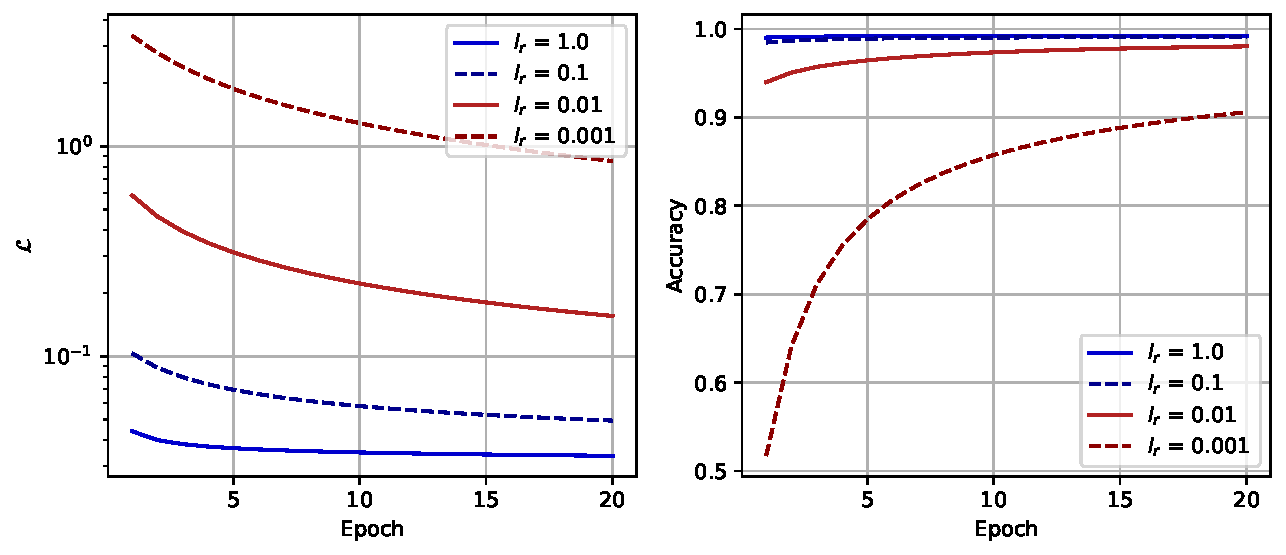
\includegraphics[width=\textwidth]{figures/loss_acc_simple200labels_valid.pdf}
        \caption{Validation dataset}
    \end{subfigure}
    \caption{Loss and accuracy.}
    \label{fig:loss_acc_simple200labels}
\end{figure}

The training of the \texttt{LSTMProteinClass} is longer than the \texttt{SimpleProteinClass} for all learning rates studied but it manages to get a rather good accuracy for $l_r = 0.1$ as shown in Fig.~\ref{fig:loss_acc_lstm200labels}.

\begin{figure}[htbp]
    \centering
    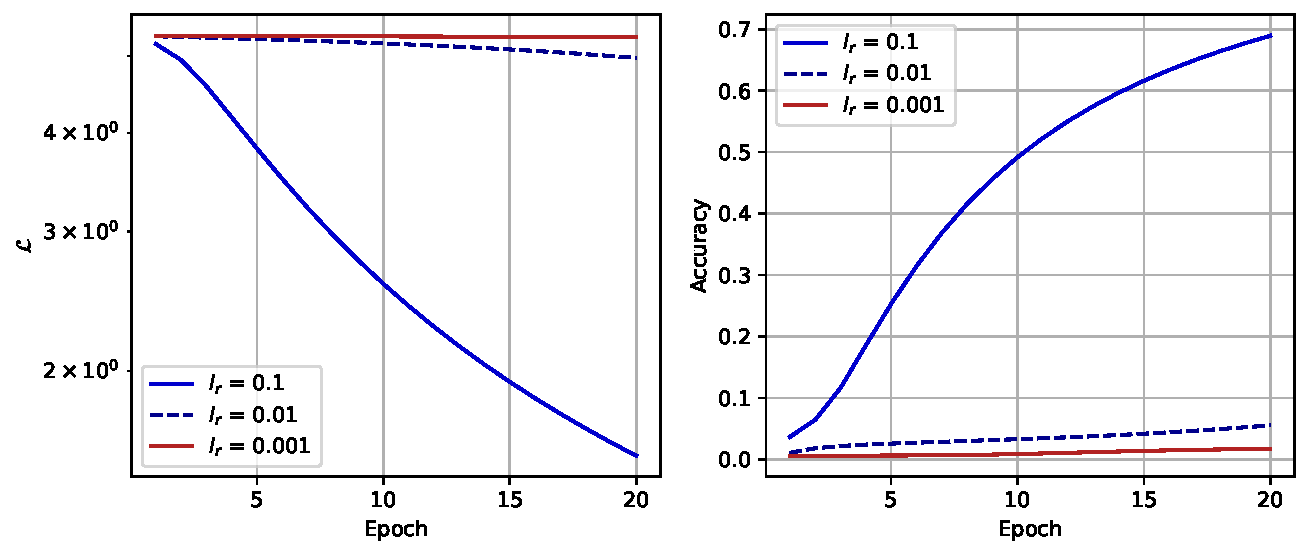
\includegraphics[width=\textwidth]{figures/loss_acc_lstm_train.pdf}
    \caption{Loss and accuracy for training dataset.}
    \label{fig:loss_acc_lstm200labels}
\end{figure}

Training of the RNN network proved to be unsuccesful. Hyperparameter tuning should be more thoroughly explored for improvement. The three best networks of each architecture are compared in Fig.~\ref{fig:networks_comp}.

\begin{figure}[htbp]
    \centering
    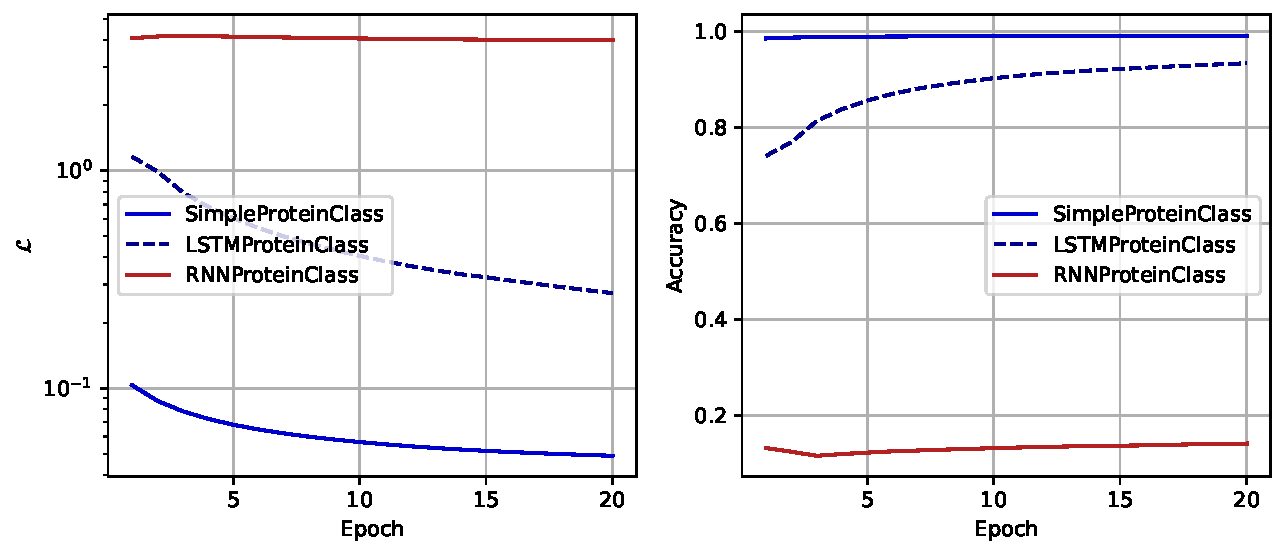
\includegraphics[width=\textwidth]{figures/networks_comp_200labels.pdf}
    \caption{Loss and accuracy for the validation dataset using the 3 different architectures.}
    \label{fig:networks_comp}
\end{figure}

\subsection{Longer sets}

We increase the number of included labels in the sets by taking into account 5000 labels which brings the data sets closer to reality (18 000 labels in the original data set). The \texttt{SimpleProteinClass} with the optimal hyper-parameters found earlier work well on these datasets as well. Increasing further the number of labels to 15 000 yield good results although training should be extended to more than 20 epochs to really get the best accuracy as shown in Fig.~\ref{fig:simple_nlabels}. The network start to get really big with respectively 20 005 840 and 60 015 840 parameters for the 5000 and 15 000 label networks respectively.

\begin{figure}[htbp]
    \centering
    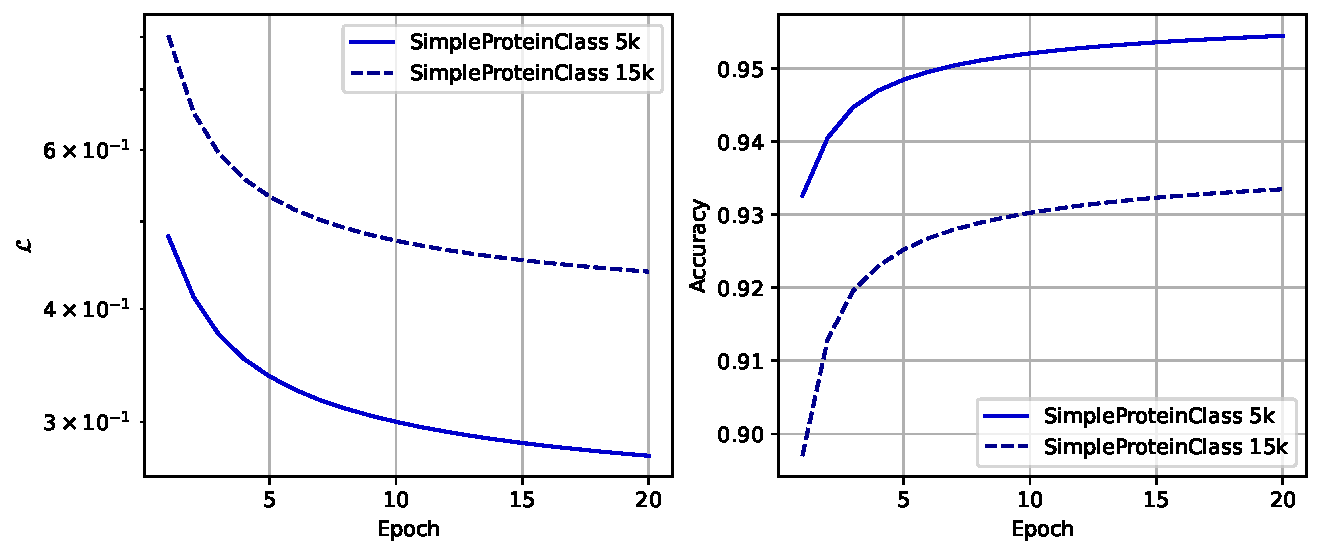
\includegraphics[width=\textwidth]{figures/loss_acc_nlabels_valid.pdf}
    \caption{Loss and accuracy for the validation dataset using 5000 and 15 000
    labels datasets.}
    \label{fig:simple_nlabels}
\end{figure}

\section{Conclusion}

A method for classifying the PFam dataset has been carried out in this document. The dataset analysis shows a certain repartition of length and amino-acids which leads to a first reduction of the dataset to homogeneize it. Restricting to only the 20 most common amino-acids the sequences, an embedding has been chosen over a one-hot encoding for each sequence. Three networks have been tested throughout this document and the simplest one has proven to yield the best results. More hyperparameter tuning is necessary for the other models to get better accuracy and could be carried out in the future.


\clearpage

\bibliographystyle{unsrtnat}
\setcitestyle{square} %round for parentheses
\bibliography{refs}

\end{document}